\chapter{Módulo 1 – Núcleo Comum de Formação (210 Horas)}
\label{chap:modulo1}

O \textbf{Núcleo Comum de Formação} constitui a base obrigatória e estruturante do programa de Residência Tecnológica Seldon. Seu propósito central é nivelar os residentes em fundamentos sólidos de engenharia de software, rigor do método científico, arquitetura de sistemas móveis, desenvolvimento Android com Kotlin moderno, testes automatizados e gestão ágil de projetos orientada a evidências.

Composto por sete disciplinas complementares que totalizam 210 horas letivas, este módulo estabelece o vocabulário conceitual e a capacitação técnica essenciais para a atuação nas três trilhas de especialização posteriores.

---

\section{Dados, Experimentação e Metodologia Científica (30h)}

\begin{pedagogico}{Objetivo Pedagógico da Disciplina}
Capacitar os residentes para formular problemas de engenharia tecnológica com rigor formal, desenhar ensaios experimentais reprodutíveis, estabelecer métricas objetivas de desempenho e interpretar evidências estatisticamente válidas, respeitando os preceitos de propriedade intelectual.
\end{pedagogico}

\subsection{Formulação de Problemas Tecnológicos e Hipóteses}
Na engenharia de software contemporânea, decisões arquiteturais e otimizações de baixo nível não podem se basear em intuição empírica desprovida de validação formal. O método científico aplicado a sistemas computacionais exige a estruturação de hipóteses estatísticas verificáveis:
\begin{itemize}
    \item \textbf{Hipótese Nula ($H_0$):} Postula que a modificação introduzida (ex.: nova estratégia de compactação de memória ou novo algoritmo de renderização) não produz diferença estatisticamente significativa no parâmetro de interesse em comparação com a linha de base (\textit{baseline}).
    \item \textbf{Hipótese Alternativa ($H_1$):} Postula que a intervenção tecnológica produz um efeito real mensurável (redução de latência, menor variabilidade temporal ou conservação de energia).
\end{itemize}

\subsection{Desenho Experimental e Variáveis de Controle}
O isolamento de ruído em plataformas móveis como o Android é um dos desafios mais complexos na coleta de métricas, devido a variáveis intervenientes não controladas:
\begin{enumerate}
    \item \textbf{Variável Independente ($X$):} O fator sob manipulação direta do pesquisador (ex.: uso de \texttt{LazyColumn} em Jetpack Compose versus \texttt{RecyclerView} tradicional).
    \item \textbf{Variável Dependente ($Y$):} A métrica de resposta observada (ex.: tempo de renderização por quadro $T_{\text{frame}}$ em milissegundos).
    \item \textbf{Variáveis de Controle e Ruído:} Fatores externos que devem ser congelados durante o ensaio:
    \begin{itemize}
        \item Nível e temperatura da bateria (para evitar \textit{thermal throttling});
        \item Frequência de clock da CPU fixada via \texttt{cpufreq} no kernel;
        \item Brilho da tela fixado e rádio celular configurado em modo avião.
    \end{itemize}
\end{enumerate}

\begin{figure}[htbp]
\centering
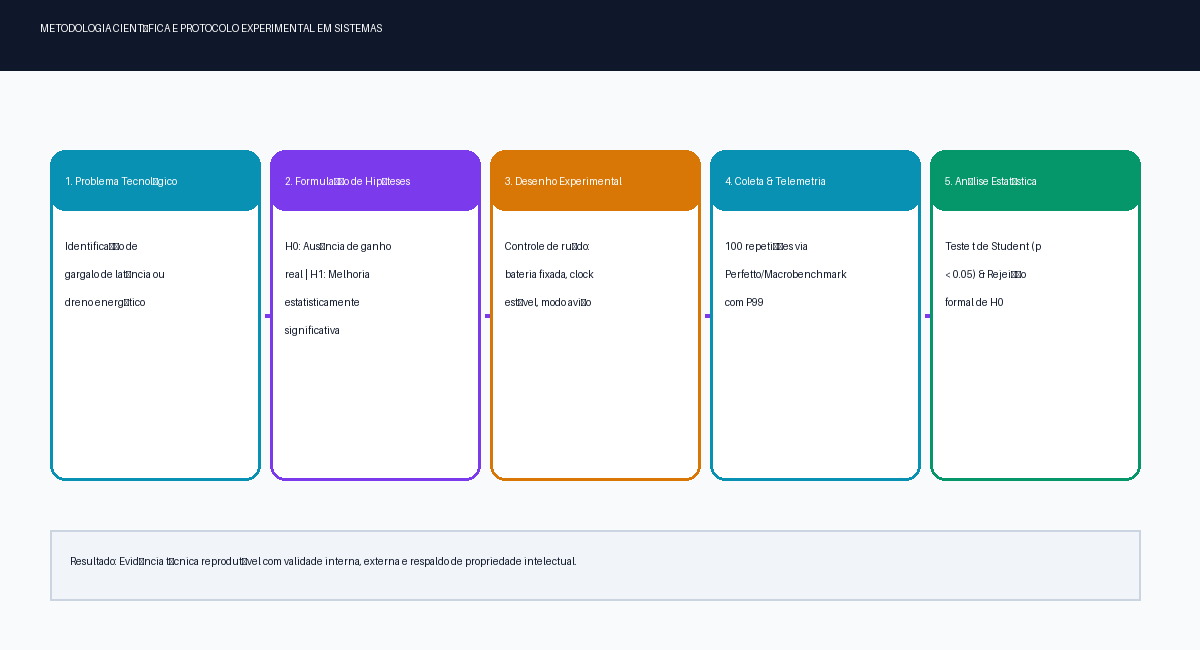
\includegraphics[width=0.95\textwidth]{imagens/fig_metodologia_cientifica.png}
\caption{Fluxograma do Protocolo Experimental Rigoroso: formulação de hipóteses estatísticas, controle de ruído térmico/clock e validação via Teste $t$ de Student ($p < 0{,}05$).}
\label{fig:metodologia}
\end{figure}

\subsection{Análise Estatística Inferencial: Teste $t$ de Student e ANOVA}
Para rejeitar formalmente a hipótese nula $H_0$ com nível de significância $\alpha = 0{,}05$, calcula-se a estatística $t$ para duas amostras independentes com variâncias populacionais desconhecidas:
\begin{equation}
    t = \frac{\bar{X}_1 - \bar{X}_2}{\sqrt{\frac{s_1^2}{n_1} + \frac{s_2^2}{n_2}}}
\end{equation}
onde $\bar{X}_i$ representa a média amostral, $s_i^2$ a variância amostral e $n_i$ o tamanho de cada lote de medição. A rejeição de $H_0$ ocorre quando o $p$-valor associado à distribuição $t$ com os respectivos graus de liberdade for estritamente menor que $\alpha$, comprovando que o ganho de desempenho não decorreu de mero acaso estocástico.

\begin{casopratico}{Caso Prático: Protocolo Experimental de Frame Jank}
\textbf{Cenário:} Comprovar se uma alteração na alocação de objetos em um loop gráfico reduz a taxa de quadros engasgados (\textit{jank frames}).\\
\textbf{Protocolo:} 100 repetições de um teste automatizado via \texttt{macrobenchmark}. Registro dos tempos no percentil 99 ($P_{99}$).\\
\textbf{Resultado:} $\bar{X}_{\text{antigo}} = 24{,}8\text{ ms}$, $\bar{X}_{\text{novo}} = 14{,}2\text{ ms}$. Estatística $t = 12{,}4$, resultando em $p < 0{,}001$. Conclusão: a hipótese nula é categoricamente rejeitada com 99{,}9\% de confiança estatística.
\end{casopratico}

---

\section{Engenharia de Software, Requisitos e Gestão do Desenvolvimento (24h)}

\begin{pedagogico}{Objetivo Pedagógico da Disciplina}
Desenvolver competências para elicitar, analisar e formalizar requisitos de software complexos, estruturar ciclos de desenvolvimento ágeis sustentáveis e assegurar a rastreabilidade bidirecional contínua entre o desafio industrial e a entrega executável.
\end{pedagogico}

\subsection{Engenharia de Requisitos Funcionais e Não Funcionais}
Em sistemas de missão crítica e plataformas embarcadas, a especificação precisa de requisitos constitui o primeiro baluarte contra falhas catastróficas:
\begin{itemize}
    \item \textbf{Requisitos Funcionais (RF):} Descrevem os comportamentos intrínsecos do software (ex.: ``O sistema deve sincronizar os dados biométricos com a nuvem a cada 15 minutos se houver conexão Wi-Fi'').
    \item \textbf{Requisitos Não Funcionais (RNF):} Estabelecem restrições de qualidade, tais como:
    \begin{itemize}
        \item Latência de resposta da interface gráfica $\le 16{,}6\text{ ms}$ em 60 Hz;
        \item Consumo de corrente em repouso com tela apagada $\le 15\text{ mA}$;
        \item Ocupação máxima em memória residente (RSS) $\le 64\text{ MB}$.
    \end{itemize}
\end{itemize}

\subsection{Matriz de Rastreabilidade de Requisitos (RTM)}
A rastreabilidade bidirecional é implementada através de identificadores unívocos que conectam cada necessidade do projeto ao seu artefato de verificação:
\begin{equation}
    \text{Desafio Industrial} \longrightarrow \text{RF/RNF} \longrightarrow \text{User Story} \longrightarrow \text{Branch/Commit} \longrightarrow \text{Teste Automatizado}
\end{equation}

\begin{lstlisting}[language=bash, caption={Estrutura de Rastreabilidade em Commits Git}]
# Formato de mensagem de commit em conformidade com RTM:
feat(power): [RF-042][REQ-BAT-09] migra polling para WorkManager com restricao de carga

- Substitui ScheduledExecutorService por PeriodicWorkRequestBuilder
- Garante execucao exclusivamente quando o device estiver carregando e em Wi-Fi
- Evita dreno em background (RNF-ENG-03)
- Testes unitarios automatizados em WorkManagerTest.kt (Cobertura 100%)
\end{lstlisting}

---

\section{Metodologia de Projetos, Ética e Habilidades Profissionais (30h)}

\begin{pedagogico}{Objetivo Pedagógico da Disciplina}
Preparar o residente para liderar e colaborar em equipes multidisciplinares sob a metodologia de Aprendizagem Baseada em Projetos (PBL), mantendo rigor ético profissional, governança de dados conforme a LGPD e documentação formal de decisões arquiteturais.
\end{pedagogico}

\subsection{Aprendizagem Baseada em Projetos (PBL) na Residência}
Diferente da pedagogia passiva tradicional, o PBL imerge os residentes em problemas reais trazidos por parceiros industriais. O ciclo de aprendizado estrutura-se em:
\begin{enumerate}
    \item \textbf{Imersão e Delimitação:} Análise do problema e formulação de perguntas norteadoras.
    \item \textbf{Planejamento e Decomposição:} Criação de \textit{Product Backlog} e definição de papéis (Product Owner, Tech Lead, Especialista em QA).
    \item \textbf{Ciclos de Prototipação e Experimentação:} \textit{Sprints} quinzenais com geração de evidências técnicas tangíveis.
    \item \textbf{Apresentação de Resultados \& Retrospectiva:} Demonstrações técnicas para bancas de avaliação acadêmica e corporativa.
\end{enumerate}

\subsection{Governança de Dados e Conformidade com a LGPD}
O desenvolvimento para dispositivos móveis envolve acesso a sensores sensíveis (GPS, câmera, microfone, identificadores de rádio). A Lei Geral de Proteção de Dados Pessoais (Lei nº 13.709/2018) impõe diretrizes estritas:
\begin{itemize}
    \item \textbf{Privacy by Design:} Anonimização na borda através de funções de dispersão criptográfica (SHA-256 com \textit{salt} local);
    \item \textbf{Minimização da Coleta:} Coleta estritamente restrita aos dados indispensáveis à execução do serviço contratado;
    \item \textbf{Relatório de Impacto à Proteção de Dados (RIPD):} Documentação formal descrevendo os fluxos de tratamento de dados e as salvaguardas tecnológicas implementadas.
\end{itemize}

---

\section{Arquitetura de Software (18h)}

\begin{pedagogico}{Objetivo Pedagógico da Disciplina}
Capacitar os residentes na aplicação de princípios SOLID, arquiteturas desacopladas (Clean Architecture, MVVM e MVI) e injeção de dependências em aplicações Android escaláveis e de alta testabilidade.
\end{pedagogico}

\subsection{Clean Architecture no Ecossistema Android}
A Clean Architecture preconiza a separação concêntrica de responsabilidades, assegurando que o núcleo de regras de negócio (\textit{Domain}) permaneça agnóstico a detalhes de infraestrutura (bancos de dados, redes e frameworks de UI):

\begin{figure}[htbp]
\centering
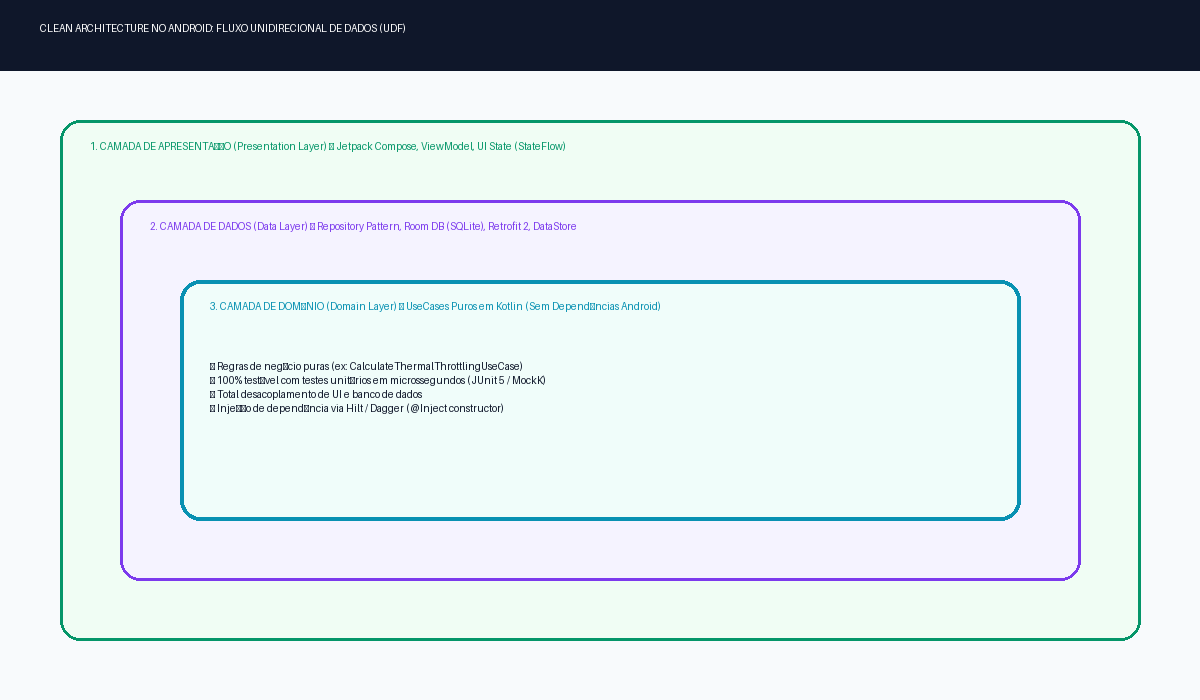
\includegraphics[width=0.95\textwidth]{imagens/fig_clean_architecture.png}
\caption{Diagrama de Camadas da Clean Architecture no Android: a camada de Domínio pura encapsulada pelas camadas de Dados e Apresentação com fluxo unidirecional.}
\label{fig:clean_arch}
\end{figure}

\subsection{Implementação Prática: UseCase Puro com Kotlin}
\begin{lstlisting}[language=Java, caption={Implementação de UseCase na Camada de Domínio}]
package com.seldon.domain.usecase

import com.seldon.domain.model.ThermalThrottlingEvent
import com.seldon.domain.repository.SensorTelemetryRepository
import javax.inject.Inject

/**
 * Regra de negócio pura: avalia risco termico sem acoplamento ao Android SDK.
 */
class EvaluateThermalRiskUseCase @Inject constructor(
    private val telemetryRepository: SensorTelemetryRepository
) {
    suspend operator fun invoke(thresholdCelsius: Double): ThermalThrottlingEvent {
        val currentTemperature = telemetryRepository.readSocTemperature()
        val isCritical = currentTemperature >= thresholdCelsius
        
        return ThermalThrottlingEvent(
            currentTemperature = currentTemperature,
            threshold = thresholdCelsius,
            requiresIntervention = isCritical
        )
    }
}
\end{lstlisting}

---

\section{Inteligência Artificial: Fundamentos, Frameworks e Aplicações (36h)}

\begin{pedagogico}{Objetivo Pedagógico da Disciplina}
Compreender a esteira completa de engenharia de Machine Learning e Deep Learning, desde a preparação de tensores de dados até o treinamento, validação cruzada, regularização e consumo de inferências preditivas integradas a aplicações móveis.
\end{pedagogico}

\subsection{O Pipeline Clássico de Aprendizado Supervisionado}
O aprendizado de máquina supervisionado visa estimar uma função $f: \mathcal{X} \to \mathcal{Y}$ que mapeie um vetor de características $\mathbf{x} \in \mathbb{R}^d$ em um rótulo $y \in \mathcal{Y}$. Em problemas de classificação, minimiza-se a função de perda de entropia cruzada (\textit{Cross-Entropy Loss}):
\begin{equation}
    \mathcal{L}_{\text{CE}}(\mathbf{w}) = -\frac{1}{N} \sum_{i=1}^{N} \sum_{k=1}^{K} y_{i,k} \log\left(\hat{y}_{i,k}(\mathbf{w})\right)
\end{equation}
onde $N$ é o número de amostras, $K$ o número de classes e $\hat{y}_{i,k}$ a probabilidade predita pelo modelo parametrizado pelos pesos $\mathbf{w}$.

\subsection{Matriz de Confusão e Métricas de Validação Rigorosas}
Em sistemas operacionais, a ocorrência de anomalias (quedas bruscas de tensão ou travamentos) representa eventos raros (dados altamente desbalanceados). A acurácia global é inadequada; priorizam-se:
\begin{equation}
    \text{Precision} = \frac{\text{VP}}{\text{VP} + \text{FP}}, \quad \text{Recall} = \frac{\text{VP}}{\text{VP} + \text{FN}}, \quad F_1\text{-Score} = 2 \cdot \frac{\text{Precision} \cdot \text{Recall}}{\text{Precision} + \text{Recall}}
\end{equation}

---

\section{Programação Java/Kotlin e Desenvolvimento de Aplicações Android (42h)}

\begin{pedagogico}{Objetivo Pedagógico da Disciplina}
Capacitar os residentes na construção de aplicações Android modernas com Kotlin, arquitetura baseada em Coroutines e Flow, interface declarativa com Jetpack Compose e domínio profundo dos quatro componentes canônicos do AOSP.
\end{pedagogico}

\subsection{Os Quatro Componentes Canônicos do AOSP}
\begin{figure}[htbp]
\centering
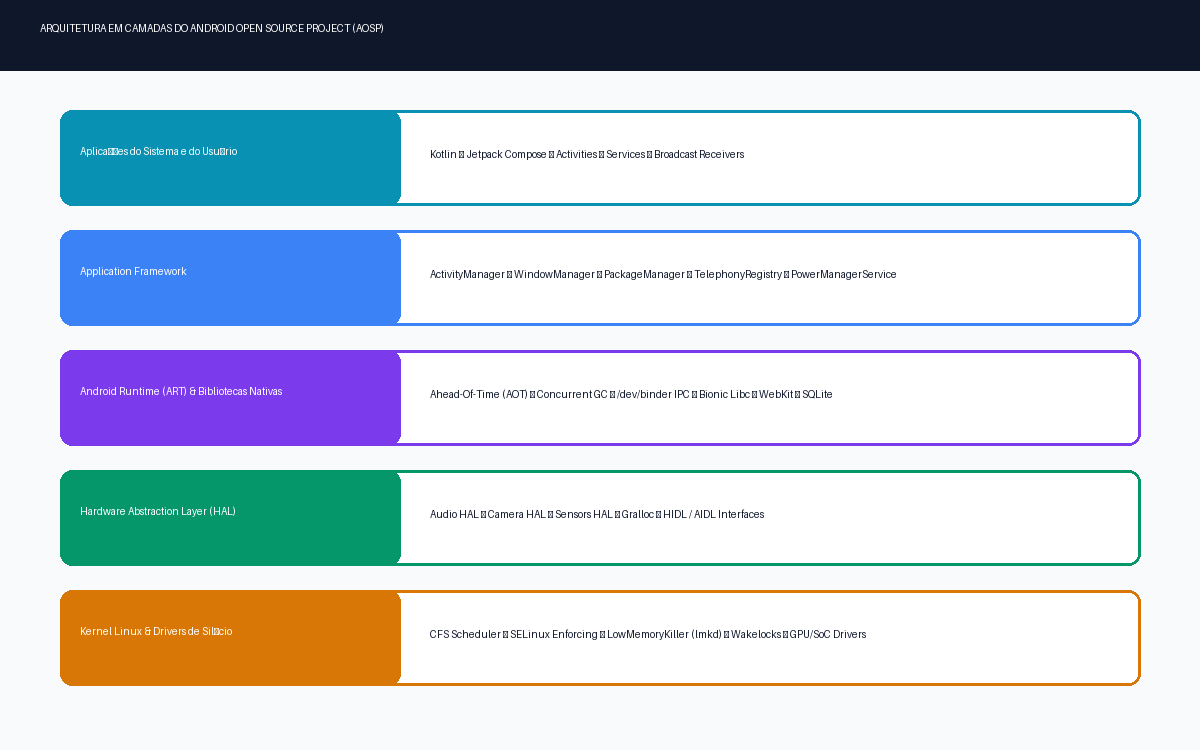
\includegraphics[width=0.95\textwidth]{imagens/fig_aosp_arquitetura.png}
\caption{Visão Geral da Pilha Arquitetural do AOSP: desde o Kernel Linux e HAL até o Android Runtime (ART) e o Application Framework.}
\label{fig:aosp_stack_cap1}
\end{figure}

O ecossistema Android fundamenta-se em quatro pilares declarados no \texttt{AndroidManifest.xml}:
\begin{enumerate}
    \item \textbf{Activity:} Representa uma interface gráfica com o usuário e controla o fluxo de vida visual (\texttt{onCreate}, \texttt{onStart}, \texttt{onResume}, etc.);
    \item \textbf{Service:} Executa processamento contínuo em segundo plano sem interface gráfica (ex.: serviços de telemetria ou reprodução de áudio);
    \item \textbf{Broadcast Receiver:} Permite à aplicação receber anúncios de eventos do sistema ou de outros apps (ex.: \texttt{ACTION\_BATTERY\_LOW}, \texttt{CONNECTIVITY\_CHANGE});
    \item \textbf{Content Provider:} Gerencia o acesso seguro e estruturado a repositórios de dados compartilhados entre processos distintos.
\end{enumerate}

\subsection{Interface Reativa com Jetpack Compose e StateFlow}
O Jetpack Compose adota o paradigma declarativo: a interface visual é uma função pura do estado atual $UI = f(State)$.

\begin{lstlisting}[language=Java, caption={Exemplo de ViewModel reativa com StateFlow em Kotlin}]
class TelemetryViewModel @Inject constructor(
    private val evaluateThermalRiskUseCase: EvaluateThermalRiskUseCase
) : ViewModel() {

    private val _uiState = MutableStateFlow<TelemetryUiState>(TelemetryUiState.Loading)
    val uiState: StateFlow<TelemetryUiState> = _uiState.asStateFlow()

    fun triggerAnalysis() {
        viewModelScope.launch {
            try {
                val result = evaluateThermalRiskUseCase(thresholdCelsius = 42.0)
                _uiState.value = TelemetryUiState.Success(result)
            } catch (e: Exception) {
                _uiState.value = TelemetryUiState.Error(e.localizedMessage)
            }
        }
    }
}
\end{lstlisting}

---

\section{Testes, Automação, Segurança e Integração Contínua (30h)}

\begin{pedagogico}{Objetivo Pedagógico da Disciplina}
Compreender e implementar esteiras de automação de testes unitários, instrumentados e de integração contínua (CI/CD), aplicando análise estática de código e boas práticas de segurança defensiva.
\end{pedagogico}

\subsection{A Pirâmide de Testes no Android}
Uma estratégia eficiente de garantia de qualidade balanceia velocidade de execução com fidelidade de ambiente:
\begin{itemize}
    \item \textbf{Testes Unitários (Base - 70\%):} Executam na JVM local em milissegundos utilizando JUnit 5 e MockK. Validam regras de negócio puras;
    \item \textbf{Testes de Integração / Robolectric (Meio - 20\%):} Simulam classes do SDK Android na JVM sem necessitar de emulador ou dispositivo físico;
    \item \textbf{Testes E2E Instrumentados (Topo - 10\%):} Executam diretamente no dispositivo via Espresso ou UIAutomator, validando fluxos críticos de ponta a ponta.
\end{itemize}

\subsection{Pipeline CI/CD Automatizado com GitHub Actions}
\begin{lstlisting}[language=bash, caption={Etapas Críticas de uma Pipeline CI/CD Android}]
# Workflow de validacao continua no GitHub Actions:
name: Android CI Pipeline
on: [push, pull_request]

jobs:
  validate:
    runs-on: ubuntu-latest
    steps:
      - uses: actions/checkout@v4
      - uses: actions/setup-java@v4
        with: { java-version: '17', distribution: 'temurin' }
      - name: Analise Estatica (Detekt & Lint)
        run: ./gradlew detekt lintRelease
      - name: Testes Unitarios
        run: ./gradlew testReleaseUnitTest
      - name: Build do APK de Release
        run: ./gradlew assembleRelease
\end{lstlisting}
